\documentclass[12pt]{article}

\usepackage{tgtermes}
\usepackage{epsf}
\usepackage{epstopdf}
\usepackage{amsmath}
\usepackage{graphicx}
\usepackage{booktabs}
\usepackage[colorlinks=true,linkcolor=blue,citecolor=blue]{hyperref}
\usepackage{dcolumn}
\usepackage{amsmath, amsthm, amssymb}
\usepackage{mwe}
\usepackage{url}
%\usepackage{harvard}
\usepackage{fancyheadings}
\usepackage{longtable}
\usepackage{authblk}
\usepackage{setspace}
%\usepackage[nomarkers]{endfloat}
\usepackage{float}
\usepackage{bbm}
%\usepackage{titling}
\usepackage{subcaption}
\usepackage{algorithm}
\usepackage{algorithmic}
\usepackage{import}
\usepackage[backend=biber,style=authoryear,
sorting=ynt,citestyle=authoryear]{biblatex}
\addbibresource{papercitations.bib}
%\usepackage[nomarkers,nofiglist,notablist]{endfloat}
\usepackage{subcaption}
\usepackage{caption}

\onehalfspacing
\textwidth 6.5in \oddsidemargin 0in \evensidemargin -0.6in
\textheight 8.5in \topmargin -0.2in

\newcolumntype{L}[1]{>{\raggedright\let\newline\\
		\arraybackslash\hspace{0pt}}m{#1}}
\newcolumntype{C}[1]{>{\centering\let\newline\\
		\arraybackslash\hspace{0pt}}m{#1}}
\newcolumntype{R}[1]{>{\raggedleft\let\newline\\
		\arraybackslash\hspace{0pt}}m{#1}}
\newcolumntype{P}[1]{>{\raggedright\tabularxbackslash}p{#1}}

\newtheorem{theorem}{Theorem}[section]
\newtheorem{corollary}[theorem]{Corollary}
\newtheorem{proposition}[theorem]{Proposition}
\newtheorem{lemma}[theorem]{Lemma}

\captionsetup{justification=centering,singlelinecheck=false}


\newcommand{\xsub}[1]{%
	\mbox{\scriptsize\begin{tabular}{@{}c@{}}#1\end{tabular}}%
}

%\renewcommand{\thetable}{\Roman{table}}

\begin{document}
	
	
	
	
	\linespread{1.2}\title{\vspace{-0.5in} Does Hospital Leadership Matter?\\ \large Evidence from Pay-for-Performance Incentives} 
	
	\date{\today}
	
	\author{\vspace{10mm}Hanna Glenn\footnote{Department of Economics, Emory University, 1602 Fishburne Drive, Atlanta, GA 30322, hanna.glenn@emory.edu.} }
	
	\maketitle
	%\setlength{\droptitle}{-10pt}
	
	\vspace{-0.2in}
	
	\singlespacing\maketitle


 \vspace{3mm}
	
    \begin{abstract}
		{\small
        In many industries, not-for-profits (NFP) are the dominant firm type. Understanding the objectives of these firms is important, but NFP firms have underlying goals that make understanding their objectives difficult. For hospitals in particular, there is mixed evidence on whether NFP hospitals differ meaningfully from for-profit (FP) hospitals. In this paper, I investigate whether leadership team composition of NFP hospitals affects how similarly they behave to for-profits. I use a novel data set on NFP hospital executives in the US (2010-2014) to investigate whether the presence of clinically trained executives affects hospital behavior. In particular, I leverage pay-for-performance initiatives in the US enacted in 2012, and measure the  readmission and mortality rate responses between FP, NFP, and NFP with and without clinically trained executives. I find that NFPs without clinically trained executives behave more like FPs than other NFPs. This is consistent with theoretical predictions if NFP hospitals with clinically trained executives value societal outcomes more than those without clinically trained executives.
		} 
	\end{abstract}
	
	
	
	
	\vspace{0.8in}
	
	\noindent Keywords: 
	
	\noindent JEL Codes: 
	
	\onehalfspacing
	
	\newpage

  The objectives and behaviors of firms that are not classic for-profits are not easily determined, and an extensive literature has sought to understand these types of firms. Not-for-profits (NFP) are thought to gain utility not solely from monetary profit, but also through accomplishing societal benefit. Researchers have speculated a variety of objective functions that could motivate NFP firms such as maximizing profit (for-profit in disguise), prestige, income, or a quality/quantity trade-off (\cite{steinberg1986revealed}). Empirical contributions to this literature center around investigating behaviors that differ between for-profit (FP), private NFP, and government firms (\cite{sloan2000not}). In this paper, I investigate whether differences in observed behavior between for-profit and not-for-profit hospitals vary differentially by leadership team composition. 
  
  Hospitals have been a common focus when seeking to understand NFP firms. This is because, first, there are different hospital ownership types within the industry, giving researchers the ability to compare the behaviors of NFPs and FPs. Second, private NFP hospitals make up 50\% of all hospitals in the US, and staff, on average, 207 beds. For comparison, FPs make up around 36\% of hospitals and staff 107 beds (\cite{ASPE_2023}). Thus, NFP behavior in the hospital industry is relevant, and directly affects consumers of health care. However, it remains unclear what objective function drives NFP hospital behavior, and whether NFP hospitals are meaningfully different from FP hospitals (\cite{sloan2000not}; \cite{erus2002inferring}; \cite{deneffe2002not}; \cite{horwitz2009hospital}). 
  
  While ownership is certainly relevant, there could be other characteristics correlated with hospital behavior independent of ownership type. Researchers have focused in particular on explaining variation in NFP behavior by the market they exist in (citations). However, I argue that an observable and economically meaningful factor is the composition top-level hospital managers. In large, publicly traded firms, executive characteristics are shown to be correlated with firm performance, indicating that there is more to firm behavior than ownership status (\cite{bertrand2003managing}; \cite{matsa2013female}; \cite{ahern2012changing}). If hospitals differ in how they value monetary profit vs. societal benefit, then ownership status certainly plays a role in these valuations, but the question remains as to whether management also plays an important role. I contribute to our understanding of hospital and NFP behaviors by investigating whether occupational background, specifically clinical training in executives, affects hospital response to pay-for-performance incentives.

  Using publicly available tax forms, I construct a novel data set of NFP hospital executives from 2009-2015. I link hospitals in this data to characteristics in the American Hospital Association (AHA) survey and Hospital Compare data. I leverage various pay-for-performance initiatives in 2012 to investigate differential hospital responses between for-profits, and NFPs with and without without clinically trained executives. 
  
  I estimate how the interaction between hospital type and post program enactment affects readmission and mortality rates. Under the assumption that hospitals would have continued to behave similarly in the absence of the programs, and that leadership teams do not change endogenously with the programs, I identify the differential response to pay-for-performance incentives by different hospital types. Among the hospitals in the data, hospitals with clinically trained executives are the minority, and differ on average from other hospitals along various dimensions. Thus, I ultimately employ synthetic difference-in-differences to analyze a group of comparison hospitals with similar characteristics to treatment hospitals.\footnote{I also present results for the full sample, and find qualitatively similar results.} 
  
   While all hospital types decrease readmission rates after the programs are enacted, NFPs with clinically trained executives respond less than both FPs and NFPs without clinically trained executives. That is, NFPs without clinically trained executives respond to incentives more similarly to FPs than other NFPs. Using changes in executive teams, I decompose this effect into signalling (clinical executives signal underlying hospital preferences), or managing (clinical executives manage the hospital differently) effects. I find that the entire difference in response is driven by a managing effect. 

    This paper contributes to three strands of literature. First, it adds to our understanding of NFP hospital objective functions. There is mixed evidence on whether NFP behavior differs from FP behavior: costs, uncompensated care, technology adoption, and quality (\cite{sloan2000not}; \cite{eggleston2008hospital}; \cite{moscelli2018effect}; \cite{moscone2020public}). To this point, researchers have found that NFPs do not act as purely profit maximizers, but maximize some combination of profit and output (\cite{deneffe2002not}, \cite{chang2011nonprofit}). A paper with an approach similar to mine which investigates hospital behavior is \citeauthor{chang2011nonprofit} (\citeyear{chang2011nonprofit}), which looks at the effect of a cost shock on likelihood of shutting down and mix of profitable services. They find that NFPs and FPs are equally as likely to shut down after the shock, but only NFPs adjust their mix of profitable services. Similarly, I investigate a change in incentives to hospitals, but I look at the differential impacts of leadership teams within not-for-profits. This paper adds to our understanding of inputs into not-for-profit hospital objective functions. 

    Second, many researchers have documented a correlation between executive backgrounds, specifically for CEOs, and firm performance, starting with \citeauthor{bertrand2003managing} (\citeyear{bertrand2003managing}), who show that manager fixed effects are an important driver of many firm behaviors and decisions. Female board members are associated with better oversight and more women executives (\cite{matsa2011chipping}; \cite{adams2009women}), but are negatively correlated with firm value (\cite{ahern2012changing}). Having more female executives is correlated with female employee wages and corporate strategies (\cite{flabbi2019female}; \cite{matsa2013female}); young male CEOs tend to be more aggressive in mergers and acquisitions, while those with military experience are less aggressive (\cite{levi2010deal}; \cite{benmelech2015military}); CEOs with general ability tend to receive higher pay and perform better (\cite{kaplan2012ceo}; \cite{custodio2013generalists}; \cite{adams2018director}; \cite{frydman2019rising}). Further, Chief Diversity Officers are not found to have any effect on hiring more diversely in universities (\cite{bradley2022impact}). 
    
    Due to data limitations, many of these studies focus on large, publicly traded firms in the US. \citeauthor{brickley2010board} (\citeyear{brickley2010board}) has the only study to my knowledge answering this question in the US NFP context. Using exogenous variation in expected Medicare profits, the authors find that having an internal board of directors increases CEO compensation, and having physician board members decreases public donations (\cite{brickley2010board}). Additionally, two studies focus on hospital performance in other countries. \citeauthor{janke2019impact} (\citeyear{janke2019impact}) uses data from England to study whether CEOs affect hospital production, and find no association (\cite{janke2019impact}). However, \citeauthor{otero2022managers} (\citeyear{otero2022managers}) investigates the role of CEOs in public hospitals and Chile, and finds an 8\% decrease in mortality rates for hospitals with top managers (\cite{otero2022managers}). I contribute to this literature by considering the executive team as a whole rather than just CEOs, by investigating a context which is not largely studied but is policy relevant, NFP US hospitals, and by leveraging a unique executive characteristic pertinent to that context. 

    Finally, I contribute to our understanding of how providers respond to pay-for-performance incentives in health care. The most in depth study of how hospitals respond to HRRP is \citeauthor{gupta2021impacts} (\citeyear{gupta2021impacts}), who finds that hospitals decreased readmissions by 5\% and mortality rates by 2\% on average as a result of the program, confirming prior studies (\cite{mellor2017does}; \cite{ziedan2018essays}; \cite{ody2019decreases}; \cite{gupta2021impacts}). Around 40\% of the decrease in readmissions is due to selective patient practices. Research on HVBP generally finds that the program had no effect on underlying hospital quality (\cite{us2015hospital}; \cite{norton2018moneyball}; \cite{friedson2019so}). This paper contributes to our understanding of how characteristics of hospitals affect response to pay-for-performance incentives. 

    

    \section{Setting}

    \subsection{Not-for-Profit Hospital Executives}

    Not-for-profit firms in the US differ from for-profits mainly in that for-profit firms distribute revenue to stakeholders, while not-for-profits reinvest profit back into the firm. An important distinction between the two is that NFPs are, in general, driven by goals to better society, and therefore receive tax benefits from the government.
    
    Hospitals are governed by a board of directors, whose role is to set broad goals and strategies, and provide general oversight. The board selects executives, the highest level of management of a firm, to carry out day-to-day operations. An executive team usually consists of at least a Chief Executive Officer (CEO) and Chief Financial Officer (CFO), but there is variation in how firms organize executive teams. It is not uncommon for hospital executives to specialize in health care settings by earning a degree in health care management, or an MBA specific to health care. There are executive positions that are often filled by someone with clinical training, such as a Chief Medical Officer (CMO), and doctors can even find themselves in other top managerial positions as well, such as CEO or president. While some doctors earn additional degrees before stepping into an executive role, this is not a necessary condition to becoming a physician executive. 

    Hiring physician executives can be controversial. On one hand, physicians bring a unique combination of clinical and administration expertise, and they have insights that can potentially improve hospital outcomes (\cite{Stajduhar_2023}, \cite{Ahmed_2022}). Alternatively, physicians may not always be adequately trained to enter into high level management positions, and therefore worsen hospital outcomes (\cite{HarvardBusinessReview2018}). 

    All tax-exempt organizations in the US are required to file a Form 990 with Internal Revenue Services (IRS) each year. There are different types of forms, but any organization grossing over \$200,000 must file the most extensive Form 990. Sections of this form include a statement of revenue, statement of functional expenses, a balance sheet, and, as used in this project, a list of all key employees, executives, and board members. Each firm is required to report the name and title, average hours per week, position, and compensation of their board members and executives. 

  
    \subsection{Pay-for-Performance Policies}\label{sec:hrrp}

    Two programs were passed as part of the Affordable Care Act that focused on pay-for-performance incentives for hospitals: the Hospital Readmissions Reduction Program (HRRP), and the Hospital Value Based Purchasing Program (HVBP). HRRP focused on penalizing hospitals with poor quality, and HVBP focused on rewarding hospitals with high quality or show improvement in quality. 

    In October 2011, the Center for Medicare and Medicaid Services (CMS) released a set of rules under HRRP mandating penalties for hospitals with above average readmission rates. A readmission is when a patient returns to the hospital within 30 days of being discharged from a previous stay; avoidable readmissions are a bad outcome for patients and increase health care spending. The goal of HRRP is to lower readmissions through better care coordination, less initial stay complications, and better post-care instructions. Beginning in October 2012, hospitals with higher readmission rates than the national average in pneumonia, heart failure, or AMI (after adjusting for demographic characteristics) receive a fixed lower reimbursement rate for all Medicare patients seen in their hospital. In 2015, CMS also included chronic obstructive pulmonary disease, coronary artery bypass graft surgery, and elective primary total hip arthroplasty and/or total knee arthroplasty as conditions which go into the penalty calculation (\cite{CMS}). 
    
    Penalties are given in the form of a fixed rate reduction of 1-3\% for every Medicare patient regardless of the condition. Further, CMS does not distinguish a necessary readmission from an avoidable readmission; any repeat hospital visit is included in the penalty calculation. Excess readmission rates are calculated using a rolling look-back period of 3 years to determine whether the hospital is penalized. Therefore, hospitals had incentive to react immediately once details of the program were announced in October of 2011. These penalties are not insignificant; penalized hospitals paid, on average, 4-5\% of revenue. 

    The HVBP Program instead rewards hospitals with high quality or significant improvement in quality. Specifically, CMS deducts Medicare payments by 2\% from all eligible hospitals, collects this sum, and divides it among the rewarded hospitals. Several quality and cost measures surrounding safety, efficiency, cost reductions, clinical outcomes, and community engagement are combined to create a single score metric for each hospital. Hospitals are then compared to the average and are rewarded for being above average quality or for showing improvement (\cite{CMS_2023}). 

    

	\section{Data}\label{sec:data}

    Hospital executive teams are understudied partly due to the inaccessibility of granular data. I construct a novel data set of not-for-profit hospitals in the US that contains names, titles, and positions of all board members and executives tied to the hospital from 2009-2015. I gather this data from publicly available Tax Form 990s, which every sufficiently large not-for-profit files each year in the US. To my knowledge, this is the first large scale gathering of executive names from these forms.\footnote{\citeauthor{brickley2010board} (\citeyear{brickley2010board}) collects compensation data for a select number of hospitals.} 

    The historical tax forms for all not-for-profits are housed by ProPublica.\footnote{https://projects.propublica.org/not-for-profits/} I use the NonProfit Explorer API to extract Employee Identification Numbers (EIN) of NFPs with a hospital National Taxonomy of Exempt Entities (NTEE) code. After filtering out associations and specialty hospitals, there are approximately 3,000 NFP EINs. Linking these EINs to other hospital information is crucial for the analysis. I therefore rely on matching by location and name of hospital in both the tax forms and AHA data. I confidently match 1200 EINs to an AHA identification number based on exact name matches within the same state. I assess the observable differences between matched and non-matched hospitals in Appendix \ref{app:matched}, and conclude that the samples are overall similar apart from an under-sampling of hospitals that belong to systems.
    
    For each of the matched EINs, I extract web URLs to Form 990 PDFs for each year. I use an algorithm to download these locally and use optical character recognition (OCR) text extraction methods to scrape the relevant section of the PDF, which is titled ``Officers, Directors, Trustees, Key Employees, and Highest Compensated Employees". Finally, I use string cleaning methods to identify all names and positions under each EIN, year. With each name, I extract titles indicating clinical training: MD, Dr., or DO. Using OCR extraction can be unreliable in cases where the text on the form is handwritten or small. Therefore, for observations that are missing after the initial extraction, I manually record names, positions, and titles. This yields 852 not-for-profit hospitals that are matched to AHA data, and are not missing text information. 

    For the purposes of this paper, I focus mainly on executive teams as a whole instead of specific positions. The main reason for this is because the organization of teams varies so drastically across hospitals that a specific position, even if it exists in two different hospitals, can be meaningfully different. Additionally, the more granular the information I extract, the more likely there will be a mistake in the OCR extraction. Thus, to preserve correctness of the independent variable of interest, I focus on whether there is any MD executive at the hospital.
    
    I drop anyone who is solely a board member, and focus on those who have executive in their title, or are labeled as a president or vice president of a department. I create various hospital-level characterizations based on their executive team, such as the existence of a clinically trained executive, the number of clinically trained executives, the number of total executives, and whether the hospital has a Chief Medical Officer. Additionally, I examine changes in propensity to hire a clinical executive. Summary statistics for these variables are shown in Table \ref{leader_sumstats}. On average, NFP hospitals in my sample have 4 executives and .4 clinically trained executives. Sixty-one percent of the sample never changes propensity to hire a clinically trained executive, and 33\% of NFPs in the sample have a Chief Medical Officer at some point. 

    \import{Tables}{leader_sumstats.tex}

    I combine the created sample of not-for-profits with all for-profits in the AHA survey. The outcomes I consider are readmission and mortality rates, which are directly targeted in the pay-for-performance policies, and are found in the CMS Hospital Compare data. I combine rates for pneumonia, AMI, and heart failure (the relevant HRRP conditions) into a weighted average based on the number of patients in each condition. Additionally, I include several relevant hospital characteristics: number of beds, whether the hospital is an academic medical center, is physician owned, or is system affiliated, all come from the AHA survey. Case mix index, a measure of overall patient complexity, comes from CMS. Whether the hospital was penalized under HRRP or received payments under HVBP is found in the HCRIS data. Finally, I limit to years 2010-2014.

    % In Table \ref{sumstats}, I present summary statistics for hospital variables. There are 3,766 total hospitals in the sample, with 150 beds on average. Hospitals in the sample are less likely to be penalized for AMI than either heart failure or pneumonia under the HRRP program. On average, 20\% of patients with one of these conditions would be readmitted. While readmission rates for the specific conditions are similar, the highest likelihood of readmission is for heart failure patients. Alternatively, AMI is the most dangerous condition in terms of mortality rates. 

    %\import{Tables}{overall_sumstats.tex}

    There are several samples of hospitals that are relevant for the analysis. First, there are all for-profits and all not-for-profits. Further, I subset the sample of NFPs into whether they have a clinical executive at some point in the sample. Finally, I characterize a NFP leadership team as being stable or not. A stable team means the hospital did not change their propensity to hire a clinical executive over time. I present a table of means for each of these sub-samples in Table \ref{tab:sumstats_samples}. Approximately 850 NFPs have leadership information, with 384 of them hiring an MD executive at some point in the sample. I compare these NFPs with the 708 for-profits from the AHA Survey. For-profits and NFPs are roughly the same bed size, but NFPs see more patients in each of the three relevant conditions. For-profits are more likely to be penalized, but also more likely to receive HVBP incentives (potentially for improvement in quality). For-profits have higher readmission rates, and higher mortality rates in all categories except heart failure. There are also key differences in not-for-profits with and without clinically trained executives. Those with MDs are larger, more likely to be penalized, have higher uncompensated care, and more complex patients. This holds for stable leadership teams as well, though the number of NFPs with a clinical executive drops significantly. I discuss the implications of these differences for identification in Section \ref{sec:model}. 

    \import{Tables}{sample_sumstats.tex}

    I plot weighted average readmission and mortality rates across time for different hospital types in Figure \ref{fig:weighted_read_mort_graph}, where I adjust both rates by baseline patient complexity. Pay-for-performance incentive changes are shown as a dotted line between 2011 and 2012. For-profit hospitals have the highest readmission rates prior to 2012. While the readmission rate trend behaves similarly across hospital types prior to the programs, there are notable trend differences after the programs. NFPs with clinically trained executives show a more mitigated decrease in readmissions compared to the other types. In mortality rates, NFPs with a clinically trained executive have the lowest rates before the programs, but differentially continue with an increasing trend in mortality after the programs. While this is purely descriptive evidence, the trends in outcomes point to more similar behavior between for-profits and NFPs without a clinically trained executive in comparison to NFPs with a clinically trained executive.

    \begin{figure}[ht!]
    \centering
        \caption{Outcomes Over Time}
        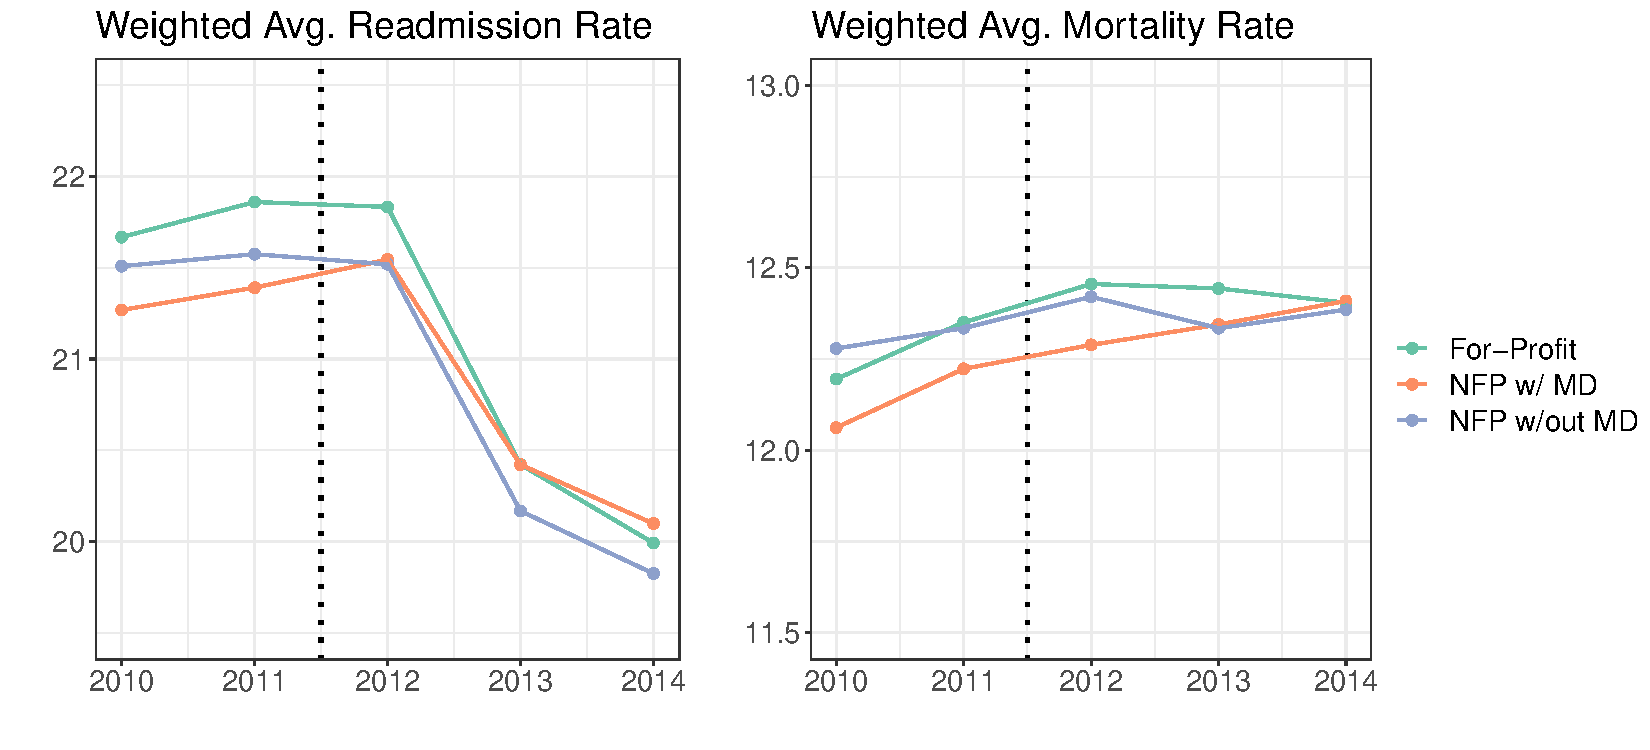
\includegraphics[width=\textwidth]{Objects/weighted_read_mort_adjusted_graph.pdf}
        \label{fig:weighted_read_mort_graph}
    \end{figure}


    \section{Model and Empirical Strategy}\label{sec:model}

    I model hospital behavior under two simplified worlds: one where quality does not directly affect profit, and one where it does. Pay-for-performance incentives essentially incorporate performance directly into a hospital's profit function. I directly model performance as quality of care, which is inversely related to readmission and mortality rates. While the literature speculates about the true form of NFP objective functions, we can generally think of hospitals choosing some linear combination of profit and societal benefit, without knowing how much weight the hospital places on each. Intuitively, a hospital that places only weight on profit (for-profit type) will only care about quality when it enters into the profit function, and therefore will respond more drastically to pay-for-performance than a hospital who already cared about quality through societal benefit before the incentives. Therefore, hospital responses to pay-for-performance incentives reveal information about their underlying preference on profit vs. societal outcomes. 

    To formalize this intuition, I specify the hospital objective function as a weighted average of profit and societal (or patient) outcomes and derive characteristics of the optimal quality. For simplicity, I abstract away from quality having a direct effect of quantity and price. Without any financial incentives to increase quality, hospital quality is decided by:  
    
    $$\max_{\theta}\hspace{2mm}\alpha\left[R - c_{\theta}(\theta) \right] + (1-\alpha) u(\theta),$$

    \noindent where $R$ is net revenue, $c_{\theta}(.)$ is an increasing cost function specific to quality $\theta$, $u(.)$ is extra utility gained from quality, which is increasing and concave in $\theta$, and $\alpha\in[0,1]$ captures the weight placed on profit vs. societal benefit. There is an implicit stay open condition throughout the model. Taking the first order condition yields 

    $$(1-\alpha)u'(\theta) = \alpha c_{\theta}'(\theta),$$

    \noindent where marginal benefit equals marginal cost of increasing quality. Solving for $u'(\theta)$ and differentiating with respect to $\alpha$:

    $$\frac{du'(\theta)}{d\alpha} = \frac{1}{(1-\alpha)^2}c_{\theta}'(\theta) > 0.$$

    \noindent Thus, by the Implicit Function Theorem, 

    $$\frac{d\theta}{d\alpha} = \frac{du'(\theta)/d\alpha}{du'(\theta)/d\theta} < 0.$$

    \noindent That is, the more weight on profit, the lower quality of care chosen by the hospital.

    In a world with pay-for-performance incentives, which can either look like benefits from high quality (such as HVBP) or penalties for low quality (as in HRRP), quality directly affects revenue. Thus, $R(\theta)$ is an increasing function of $\theta$, and I assume that the marginal financial benefit of increasing quality is greater than the marginal cost ($R'(\theta)\geq c_{\theta}'(\theta))$. Thus, the new first order condition yields:

    $$u'(\theta) = \frac{\alpha}{1-\alpha} \left[c_{\theta}'(\theta)-R(\theta)\right] \leq 0.$$

    \noindent Taking the derivative of this with respect to $\alpha$,

    $$\frac{du'(\theta)}{d\alpha} = \frac{1}{(1-\alpha)^2}c_{\theta}'(\theta).$$

    Therefore, again using the Implicit Function Theorem,

    $$\frac{d\theta}{d\alpha} = \frac{du'(\theta)/d\alpha}{du'(\theta)/d\theta}\geq0.$$

    That is, all else equal, in a world with financial incentives on quality, quality is increasing with more weight placed on profit. I combine the results found in each scenario into one response function that depends on $\alpha$, where $\theta_2$ is quality under pay-for-performance incentives and $\theta_1$ is quality with no financial incentive to quality. That is, 

    \begin{align*}
        \frac{d\Delta\theta}{d\alpha}&=\frac{d(\theta_2-\theta_1)}{d\alpha}\\
        &=\frac{d\theta_2}{d\alpha}-\frac{d\theta_1}{d\alpha}\\
        &\geq 0.
    \end{align*}


    Hence, this model predicts that change in quality depends on how much weight the hospital places on profit vs. societal benefit. Particularly, hospitals with more weight on profit respond more than hospitals with more weight placed on societal benefit. In reality, $\alpha$ is unknown, except in the case of for-profits, who have revealed that they have a high $\alpha$ by their ownership status. However, not-for-profit behavior on average does not bring much clarity about their objectives. An observable and economically relevant characteristic of a hospital that could affect $\alpha$ is composition of their executive leadership team. Thus, I compare the response of for-profits and not-for-profits with different leadership teams to bring clarity on how this might point to underlying $\alpha$.
    

    \subsection{Estimation}

    In light of the theoretical predictions, I test empirically whether different hospital types respond to pay-for-performance incentives differently. I present here linear models with a two-way fixed effects specification. Ultimately, I employ synthetic difference-in-differences, which is estimating the same model with weights that more heavily factor similar trending control groups and time periods. However, for clarity, I present the unweighted specification:

    \begin{equation}
    \label{eq:forprofit}
    y_{ht} = \beta \text{ treat}_{ht} + \gamma_{h} + \delta_t + \epsilon_{ht},
    \end{equation}
    

    \noindent where $y_{ht}$ is one of the outcome variables discussed in Section \ref{sec:data}, and $\gamma_h$ and $\delta_t$ are hospital and time fixed effects, respectively. The independent variable of interest, treat$_{ht}$, captures the effect of being a certain hospital type after incentives changed in 2012. That is, I interact an indicator for hospital type with an indicator for year post 2012 for various hospital types. First, I define treat so that for-profit hospitals are being compared to subsets of not-for-profits (by limiting the sample to the relevant treatment and comparison group). Then, I limit to only not-for-profits and define treat as those without a clinical executive. Specifically, I define treat$_{ht}$ and limit the sample in four ways, shown in Figure \ref{fig:spec}. 

    An important distinction is whether the classification of NFPs by leadership team is time-varying. For overall ownership status, switching is rare, and I limit to those who never switch. However, hospital executive teams are dynamic, and whether or not a hospital employs a clinically trained executive in each period may change. Therefore, I first present effects of having a clinically trained executive among stable executive teams, i.e., NFPs with no change in their propensity to hire a clinically trained executive. 

\begin{figure}[ht!]
    \begin{center}
    \caption{\label{fig:spec}Treated and Comparison Groups}
 \begin{tabular}{| m{18em} |}
 \hline
 Combination 1:\\ [0.5ex]
 \hline\hline 
 \vspace{2mm}
 Treat Group: \hspace{23.5mm} For-Profit \\
 \vspace{2mm} 
 Comparison Group: \hspace{11.5mm} Stable NFPs  \\
 [1ex]
 \hline
 \end{tabular}
\hfil   %<---
 \begin{tabular}{|m{18em}|}
 \hline
 Combination 2:\\ [0.5ex]
 \hline\hline
 \vspace{2mm}
 Treat Group: \hspace{13.5mm} For-Profit \\
 \vspace{2mm}
 Comparison Group: \hspace{1.5mm} Stable NFP w/out MD  \\
 [1ex]
 \hline
 \end{tabular}
 
\medskip

\vspace{2mm}


  \begin{tabular}{|m{18em}|}
 \hline
 Combination 3:\\ [0.5ex]
 \hline\hline
 \vspace{2mm}
 Treat Group: \hspace{17mm} For-Profit \\
 \vspace{2mm}
 Comparison Group: \hspace{5mm} Stable NFPs w/ MD  \\
 [1ex]
 \hline
 \end{tabular}
\hfil   %<---
  \begin{tabular}{|m{18em}|}
 \hline
 Combination 4:\\ [0.5ex]
 \hline\hline
 \vspace{2mm}
 Treat Group:  \hspace{13mm} Stable NFPs w/out MD \\
 \vspace{2mm}
 Comparison Group:  \hspace{1mm} Stable NFPs w/ MD  \\
 [1ex]
 \hline
 \end{tabular}
 \end{center}
 \end{figure}


    Additionally, under certain assumptions that I discuss in Section \ref{sec:identification}, using executive team changes can be advantageous in better understanding underlying hospital motives. There are two mechanisms to having a clinically trained executives affecting outcomes: first, a clinically trained executive could be a signal of the underlying weight placed on profit, $\alpha$. Second, hiring a clinically trained executive who carries out day-to-day operations in a distinct way effectively changes $\alpha$. Thus, I also define treat and limit the comparison group in such a way that decomposes the two. Without limiting to stable teams, I consider hospitals that ever hire a clinically trained executive vs. hospitals that have a clinically trained executive in 2012 when the programs took place. These variations of Equation \ref{eq:forprofit} are shown in Figure \ref{fig:decomp_spec}.

    \begin{figure}[ht!]
    \begin{center}
    \caption{\label{fig:decomp_spec}Decomposition Model Specification Details}
 
 \begin{tabular}{| m{18em} |}
 \hline
 Decomposition 1:\\ [0.5ex]
 \hline\hline 
 \vspace{2mm}
 Treat Group:  \hspace{15mm} NFP w/out MD \\
 \vspace{2mm}
 Comparison Group: \hspace{3mm} NFPs w/ MD  \\
 [1ex]
 \hline
 \end{tabular}
\hfil   %<---
 \begin{tabular}{|m{18em}|}
 \hline
 Decomposition 2:\\ [0.5ex]
 \hline\hline
 \vspace{2mm}
 Treat Group: \hspace{11mm} No MD Exec 2012 \\
 \vspace{2mm}
 Comparison Group:  NFPs w/ MD (not 2012)  \\
 [1ex]
 \hline
 \end{tabular}
 
\end{center}
 \end{figure}

    \subsection{Identification}\label{sec:identification}

    To identify the causal effect of hospital type on hospital program response, I rely on several assumptions. First, I assume that, absent the program enactments, treat and comparison group types would have behaved similarly in outcomes. While I see no evidence of pre-trends, Table \ref{tab:sumstats_samples} suggests that hospitals with a clinically trained executive are different than other hospitals along multiple characteristics. There may be concern that these differences between hospital types could be driving the results. Therefore, my main specification uses the synthetic difference-in-differences method established in \citeauthor{arkhangelsky2021synthetic} (\citeyear{arkhangelsky2021synthetic}). This method creates unit weights that more heavily factor comparison hospitals that are similar to the treat group hospitals prior to the programs. It also weighs time periods that balance pre-programs and post-programs for the comparison hospitals. Then, a simple two way fixed effects estimator is used with these weights, yielding a more robust average treatment effect that relies less on a strong parallel trends assumption (\cite{arkhangelsky2021synthetic}). I present the synthetic diff-in-diff estimates as the main results, and they are largely similar to the standard two way fixed effects results with no weights, shown in Appendix \ref{app:fullsample}. Further, the conceptual identification is the same as a standard difference-in-differences.

     Second, I assume that executive teams are not determined endogenously with the programs. In the main specification, I limit the sample to hospitals with executive teams that do not change their propensity to hire a clinical executive over time. Thus, I rely on this sample selection not being correlated with the program enactment. In supplementary analyses, I leverage executive team changes to disentangle signalling vs. managing effects, which is only identified if leadership changes are uncorrelated with the policies. 

     I assess the validity of this assumption in two ways. First, I analyze whether changes in clinically trained executives occur more often in time periods of program enactment. Second, I analyze whether hospitals who end up getting penalized or receiving payments are more likely to make changes in clinical executive members than those who are not. That is, are hospitals that expect to be affected by the programs more likely to hire or fire clinically trained executives? I consider changes in having any clinically trained executive, as well as changes in the number of clinically trained executives. I estimate the following linear equations:

    \begin{equation}\label{eq:change1}
    \text{change}_{ht} = \sum_{j=2011}^{2014}\beta_j\mathbf{1}\{t=j\} + \alpha_h + \epsilon_{ht},
    \end{equation}

    \begin{equation}\label{eq:change2}
    \text{change}_{ht} = \beta(\text{Program Exposed}_{h} \times \text{Post Programs}_t)+ \alpha_h + \delta_t + \epsilon_{ht}.
    \end{equation}

    The variable $\text{Program Exposed}_{h}$ is an indicator for whether the hospital eventually was penalized under HRRP or received payments under HVBP. The estimates from this analysis are presented in Table \ref{tab:change_analysis}. Changes in any clinically trained executive are less likely to occur in 2012-2014 relative to 2010, indicating that executive teams are actually becoming more stable over time along the dimension of hiring clinically trained executives. Further, hospitals who end up being penalized through HRRP or receiving payments through HVBP are not more likely to change their propensity to hire any clinically trained executive. Results are similar when considering changes in the number of clinically trained executives. Thus, it seems unlikely that endogenous team formation is biasing the estimates.

     \import{Tables}{change_analysis.tex}

    Finally, I assume that no other unobserved changes occurred in 2012 that are correlated with both hospital performance and type. 

    
    
    \section{Results}

     The estimated difference in readmission rate trends for all hospital types in response to the programs are shown in Figure \ref{fig:read_synth_plot}. Each panel corresponds to a particular definition of the treat group of hospitals and limitation of comparison group hospitals.
     
     Panel \ref{fig:read_synth_plota} compares readmission rate responses among for-profits and all NFPs, and shows that on average, there is no difference in how these types of hospitals change readmission rates in response to the incentive changes. However, when the comparison group is limited to NFPs with a clinical executive, panel \ref{fig:read_synth_plotb} shows that there is a differential response to the program between these hospital types. In particular, for-profits decrease readmission rates by .3 more than NFPs with a clinical executive, an additional 3 patient readmission decrease relative to the average number of patients. While numerically small, this difference in response is non-existent between for-profits and NFPs without a clinical executive (panel \ref{fig:read_synth_plotc}), indicating some, if minor, differences in objectives resulting from having a clinical executive. 


     \begin{figure}
     \caption{Readmission Rate Synthetic Difference in Differences Results}
     \centering
          \begin{subfigure}[b]{0.45\textwidth}
         \centering
         \caption{For-Profit and All NFP}
         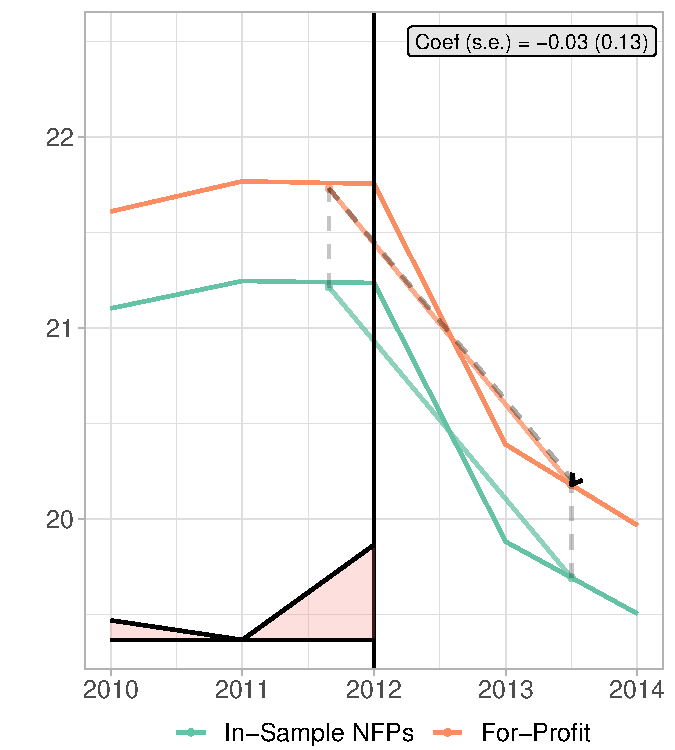
\includegraphics[width=\textwidth]{Objects/read_fp_nfp_synth_graph.pdf}
         \label{fig:read_synth_plota}
     \end{subfigure}%
     \hfill
     \begin{subfigure}[b]{0.45\textwidth}
         \centering
         \caption{For-Profit and NFP w/ MD Exec}
         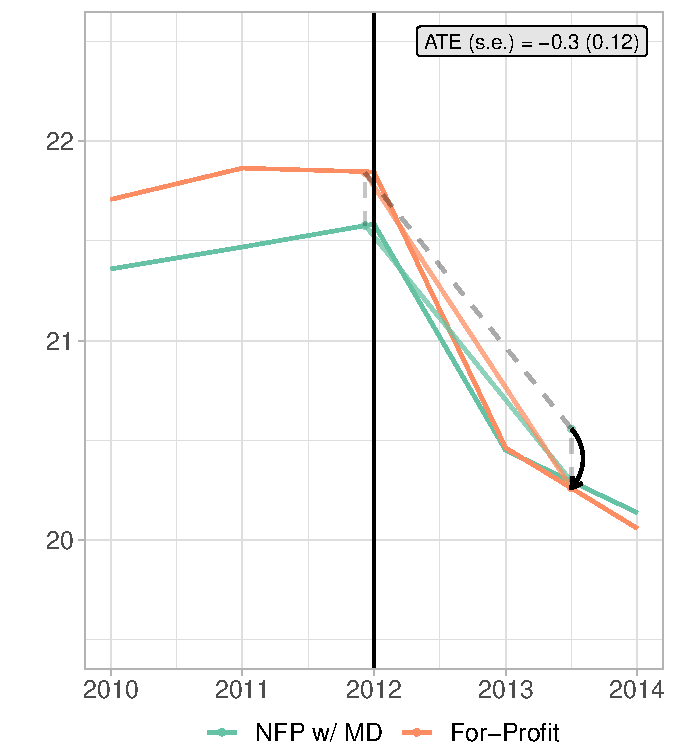
\includegraphics[width=\textwidth]{Objects/read_fp_md_synth_graph.pdf}
         \label{fig:read_synth_plotb}
     \end{subfigure}%
     \vspace{5mm}
     \hfill
     \begin{subfigure}[b]{0.45\textwidth}
         \centering
         \caption{For-Profit and NFP w/out MD Exec}
         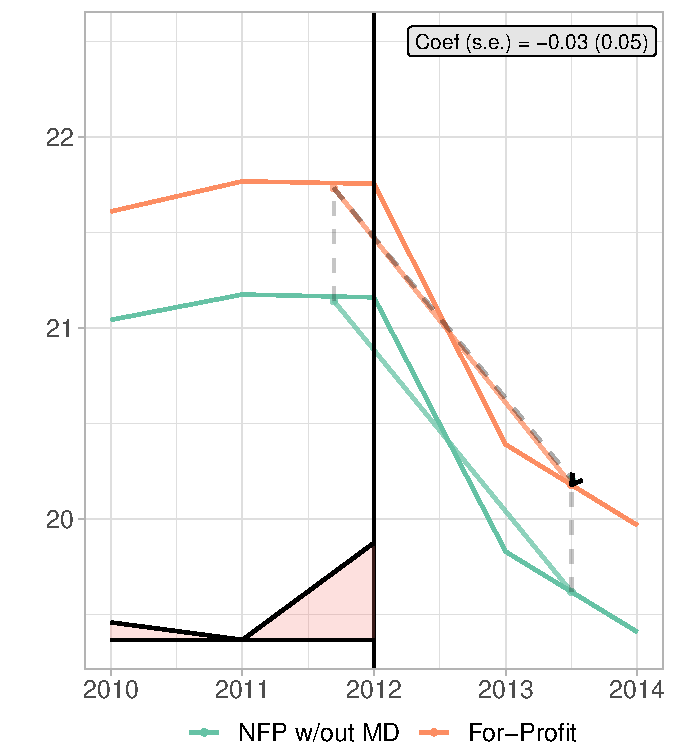
\includegraphics[width=\textwidth]{Objects/read_fp_nomd_synth_graph.pdf}
         \label{fig:read_synth_plotc}
     \end{subfigure}
     \hfill
     \begin{subfigure}[b]{0.45\textwidth}
         \centering
         \caption{NFP w/ and w/out MD Exec}
         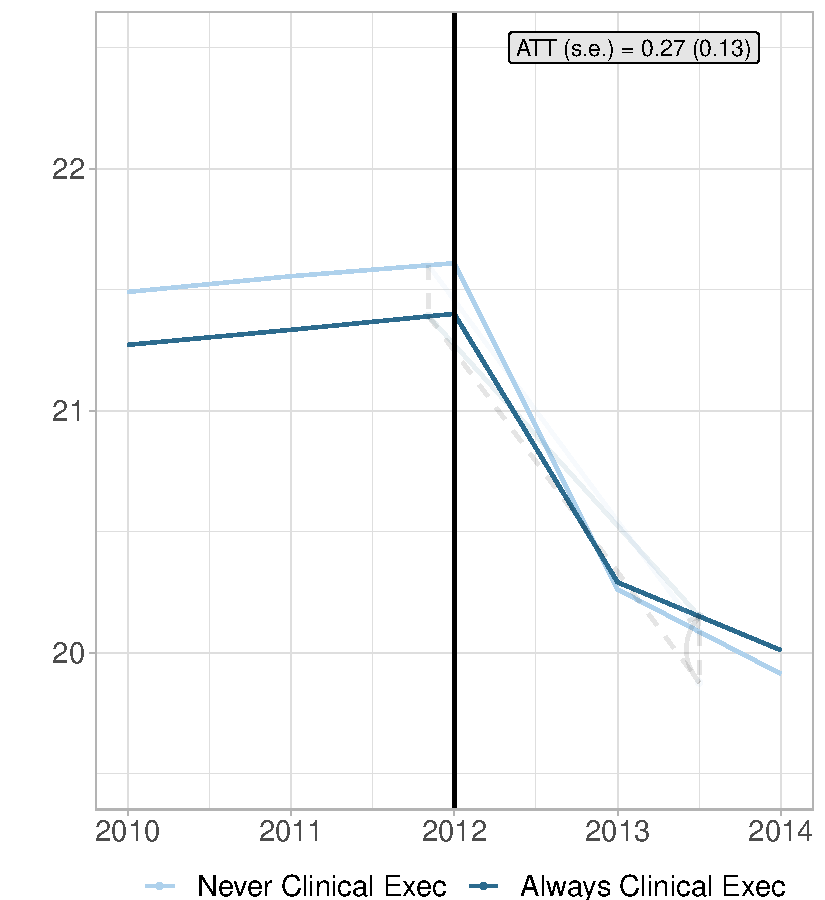
\includegraphics[width=\textwidth]{Objects/read_md_nomd_synth_graph.pdf}
         \label{fig:read_synth_plotd}
     \end{subfigure}
        \label{fig:read_synth_plot}
    \end{figure}

    Next, in panel \ref{fig:read_synth_plotd}, I directly compare NFPs with and without a clinical executive. NFPs without a clinically trained executive lowered readmission rates by .24 ppts more than NFPs with a clinically trained executive. 

    I now shift to discussing differential responses of mortality rates. I present estimated differences in mortality rates between different hospital types in Figure \ref{fig:mort_synth_plot}. Panel \ref{fig:mort_synth_plota} compares for-profit and all NFP mortality rates after the pay-for-performance incentives. These results show that there is no difference, both statistically and in magnitude, between mortality rates of for-profits and not-for-profits after the programs. This result holds when the comparison group is limited to NFPs without a clinical executive (panel \ref{fig:mort_synth_plotc}). However, when comparing for-profits to NFPs with a clinical executive, the magnitude of the difference in mortality trends jumps to -.11. While still statistically insignificant, I argue that this still indicates a difference in behavior between the hospital types, particularly due to the documented noisiness of mortality measures (\cite{mackenzie2016measuring}). 

     \begin{figure}
     \caption{Mortality Rate Synthetic Difference in Differences Results}
     \centering
          \begin{subfigure}[b]{0.45\textwidth}
         \centering
         \caption{For-Profit and All NFP}
         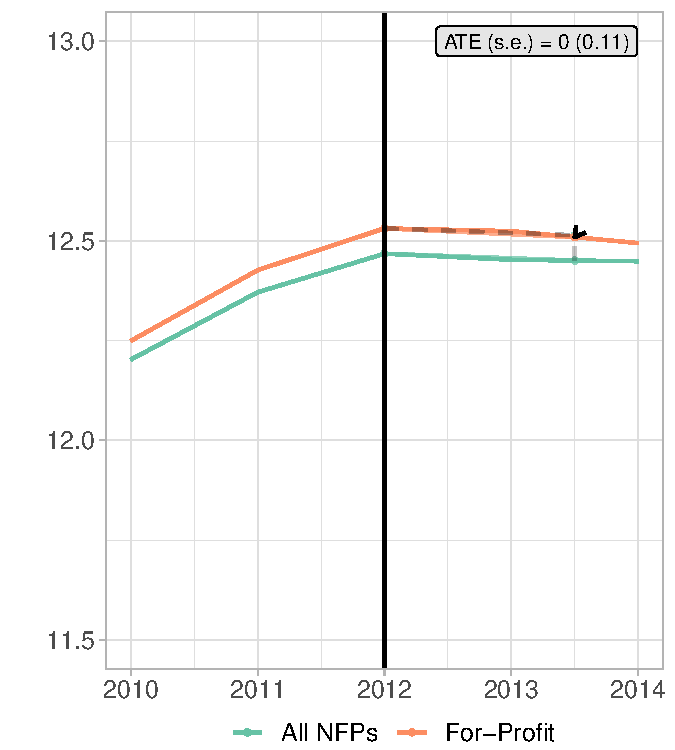
\includegraphics[width=\textwidth]{Objects/mort_fp_nfp_synth_graph.pdf}
         \label{fig:mort_synth_plota}
     \end{subfigure}%
     \hfill
     \begin{subfigure}[b]{0.45\textwidth}
         \centering
         \caption{For-Profit and NFP w/ MD Exec}
         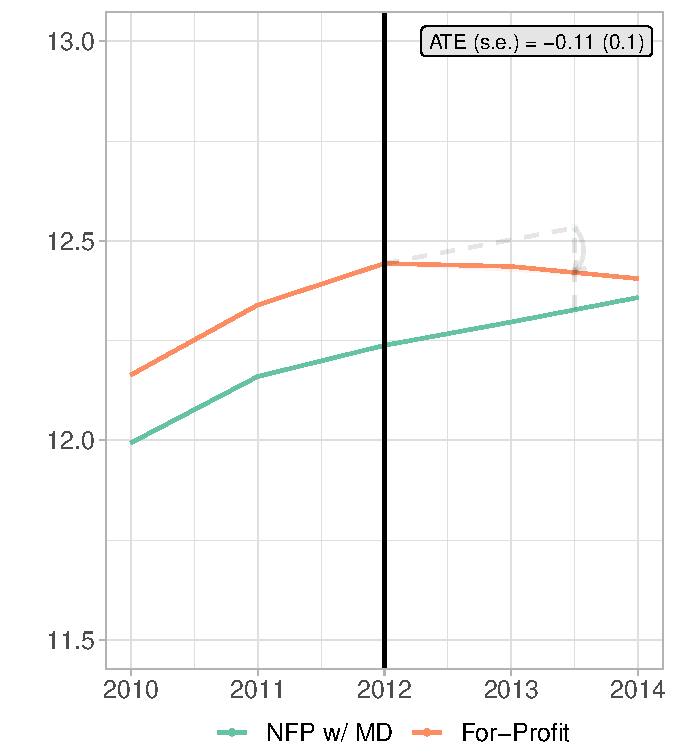
\includegraphics[width=\textwidth]{Objects/mort_fp_md_synth_graph.pdf}
         \label{fig:mort_synth_plotb}
     \end{subfigure}%
     \hfill
     \begin{subfigure}[b]{0.45\textwidth}
         \centering
         \caption{For-Profit and NFP w/out MD Exec}
         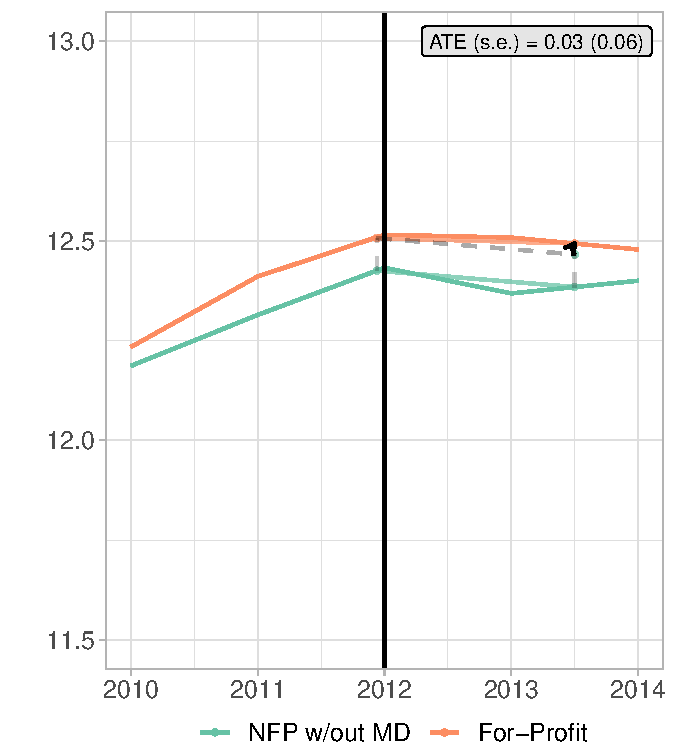
\includegraphics[width=\textwidth]{Objects/mort_fp_nomd_synth_graph.pdf}
         \label{fig:mort_synth_plotc}
     \end{subfigure}
     \hfill
     \begin{subfigure}[b]{0.45\textwidth}
         \centering
         \caption{NFP w/ and w/out MD Exec}
         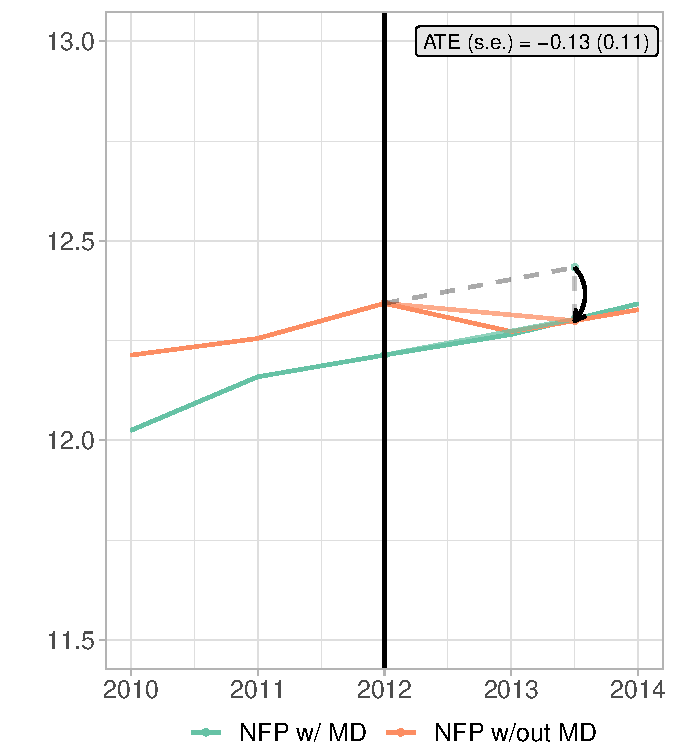
\includegraphics[width=\textwidth]{Objects/mort_md_nomd_synth_graph.pdf}
         \label{fig:mort_synth_plotd}
     \end{subfigure}
        \label{fig:mort_synth_plot}
    \end{figure}

    I also directly estimate the difference in mortality rates among NFPs with and without clinical experience in panel \ref{fig:mort_synth_plotd}. Again, the difference is not statistically significant, but the coefficient compared to the true nulls in panels \ref{fig:mort_synth_plota} and \ref{fig:mort_synth_plotc} indicates NFPs without a clinical executive potentially decrease mortality more aggressively than NFPs with a clinical executive. 

    \subsection{Decomposition}

    In the above analysis, I show that NFPs with a clinical executive seem to respond to incentives differently than both for-profits and NFPs without a clinical executive, suggestive evidence of differential objectives correlated with leadership teams. However, the analysis to this point does not speak to the mechanism by which clinical executives lead to differential behavior. In this section, I present two theories by which a clinical executive leads to differential behavior, and present descriptive evidence that one dominates the other. 
    
    First, having a clinical executive could be a signal of underlying hospital objectives. Alternatively, hiring a clinical executive could actually change the objectives of the hospital for the time the clinical executive is actively managing the hospital. To disentangle the two, I use variation in the timing of having a clinical executive, with either existence of a hospital executive at any point in time, or whether the hospital has a clinically trained executive in 2012 when the programs were enacted. The results are shown in Table \ref{tab:MD_noMD_readmort_decomp_synth}. Columns (1) and (2) show that the difference in readmission response is driven by having a clinically trained executive in 2012, compared to having a clinically trained executive at another point in time. Columns (3) and (4) support the same theory given the magnitudes of the coefficients, but are still statistically insignificant due to the noisiness of mortality. The results suggest that managers make a difference in behavior and objectives, rather than being a signal of already existing objectives. 

    \import{Tables}{MD_noMD_readmort_decomp_synth.tex}

     
 

    \section{Conclusion}

    Existing literature is inconclusive as to whether not-for-profit (NFP) hospitals differ meaningfully from for-profit hospitals. NFP objectives have direct implications for patients, yet are largely unknown. An observable and economically meaningful characteristic of NFP hospitals that may affect underlying objectives is the composition of the hospital's top management. Particularly, whether any executives at the hospital have a background in practicing medicine.

    In this paper, I study differential responses to a change in incentives between for-profit and NFP hospitals with and without a clinical executive. I do this by collecting a novel data set on hospital executives from Tax Form 990s and merging this to existing hospital data. I then use a synthetic difference-in-differences methodology to estimate differential responses in readmission and mortality rates after several pay-for-performance initiatives are enacted in the US in 2012. 
    
     When comparing for-profits to all not-for-profits, I find no difference in behavior after the policies take effect, which aligns with suggestions that NFPs are for-profits in disguise. However, when I compare for-profits to NFPs with clinical executives, the two types of hospitals respond differently to the incentives. Specifically, all firm types decrease readmissions, but NFPs with a clinical executive are less aggressive in their responsiveness than the other firm types. A similar result holds for mortality rates. This finding is consistent with the theoretical prediction that firms who place more weight on societal benefit than on profit will have a more mitigated response to policies that affect profit. Additionally, under the assumption that executive team changes are not correlated with the program, I find that the differential response is driven by the actual management of the clinical executive, not by a clinical executive being a signal of underlying objectives. 
     
     These findings are informative for policymakers predicting how hospitals will responsd to a change in incentives. Specifically, they suggest that policymakers should take into account more than just ownership status when evaluating how hospitals will respond to policy changes. 

	
	\newpage

    \printbibliography

\appendix

 \section{Data}\label{appendixdata}

\subsection{Gathering Hospital Leadership Names}

I use the Nonprofit Explorer API to access the archive of NFP tax form 990s. At the time of writing this, information on using version 2 of the API can be found at \hyperlink{https://projects.propublica.org/not-for-profits/api}{https://projects.propublica.org/not-for-profits/api}. 
    
There are over 1.5 million not-for-profit entities in the US, making it crucially important to be able to filter by type of entity before analyzing any PDFs. The API allows this by filtering a query based on National Taxonomy of Exempt Entities (NTEE) code. I query only not-for-profits categorized as E20 (hospitals), E21 (community health systems), and E22 (general hospitals). The API has a pagination limit of 100, meaning I can only pull information on 100 hospitals at a time. Therefore, I filter the query further to only consider one state at a time. The only state that has more than 100 entities registered is California, and thus I subset the California query even further by names that include the word "hospital" and names that don't. I combine all of these subsets and have information on each not-for-profits Employee Identification Number. There are 5,588 EINs total in this list. This acts as a list of entities for which I can pull more information. 

I loop through the list of EINs found in the previous step and query more detailed information from the API on that specific EIN. I save the name, secondary name, state, and zip code, all of which do not vary by year. I also save each year's URL link to the Tax Form 990 PDF. For the sake of a comprehensive data set, I keep years 2006-2020 (I later limit to 2010-2014 when focusing on pay-for-performance initiatives in 2012). Thus, I finish this step with a panel data set of EIN characteristics and PDF locations. Importantly, there are multiple types of Tax Form 990s depending on the size of the not-for-profit. In many cases, one not-for-profit has at least two different forms filed in a given year. I filter out any EIN-years for which there are no PDFs on file. The data on PDF locations contains 4,012 EINs and 61,363 EIN-year-tax forms.

It is necessary to link these not-for-profits with other sources of data to recover penalties from HRRP, payments from HVBP, bed size, and outcomes of interest. The ideal hospital data set to match to is American Hospital Association (AHA) Survey, which contains hospital characteristics and Medicare ID number. However, an EIN to AHA ID crosswalk does not exist. Therefore, I take a conservative approach to matching EINs to American Hospital Association (AHA) ID based on hospital name and location. First, I will discuss limitations and cleaning of the AHA data and tax form data. 

In the AHA data, I filter only to hospitals in the contiguous US, Alaska, and Hawaii (excluding places like Puerto Rico), classified as not-for-profit or state/community, and those that are general acute care. I also filter out any hospitals who weren't present in the data (or change system ID) in 2009-2015, meaning they either closed or were acquired. Due to the survey nature of this data, a hospital name may look slightly different from one year to the next. For example, ``Waldo County General Hospital" is also ``Waldo County General Hospital Maine Health". Further, zip codes may change by one or two digits, making them unreliable to match based on. To deal with this, I first keep only unique AHA ID, name, zip, state, and system name combinations. Then, I convert the data from long to wide so that each AHA ID occurs only once, but may have multiple names, zip codes, or system names associated with it.

I consider which not-for-profit entities are not likely to be hospitals and drop them. There are numerous foundations or auxiliary firms with the purpose of raising funds for the hospital, but do not provide services to patients. I filter out any not-for-profit with "foundation" or "auxiliary" in the name. I also filter out various specialty centers that fell into the general hospital category, such as hospice or cancer centers. 

I then proceed matching based on names in multiple layers. I focus on exact string matches, so I remove all spaces and common characters that could cause mismatches such as \&, ', -, and inc. Next, I take each AHA name and look for exact matches in a not-for-profit's first or secondary name for not-for-profits in the same state as the AHA hospital. When an exact match is found, I record the link between AHA ID and EIN. In this first layer of matching, 860 hospitals in the AHA data are linked to an EIN, equivalent to 31\% of AHA not-for-profit hospitals in the sample. 

In the next layer of matching, I remove common words such as "healthcare", "regional", "hospital", etc. That way if there are subtle differences in names, removing common words may allow for an exact match. Again, I take each AHA hospital name and look for exact matches in the not-for-profits within the same state. This adds an additional 90 hospital matches, accounting for a total of 34.5\% of AHA hospitals. Finally, I manually search through unmatched EINs to identify any matches. From google searches, I identify an additional 300 EIN-AHA ID matches.

I then extract the names of board members and executives from the Tax Form 990 PDFs of matched hospitals. In the data set of hospital PDF URLs that I collected earlier, I limit to the hospitals with solid matches described above. I then loop through each EIN, downloading PDFs locally and using the tesseract package in R to extract text from the relevant pages of the PDF using OCR text extraction methods. In particular, I loop through each page of the PDF, look for the title associated with leadership names: ``Officers, Directors, Trustees, Key Employees, and Highest Compensated Employees", and save all the text from any pages where this title is found. I save the text to a list of all EIN, years present. 

One tricky aspect of the NonProfit Explorer API is that, only in some cases, if two forms are present for an EIN, year, only the first one (which is typically not the one with the relevant information) is pulled. Therefore, for some hospitals, a couple years will have gaps in text extraction data. I locate EIN, years where this problem is occurring, and a team of RAs locates and downloads the correct forms manually. I extract text from these manually downloaded forms in the same manner as above. 

The form of the text data is a data frame with one column, where each line of text is saved in a different row. Typically on the same page as the names and positions is a list of the highest compensated employees and their compensation. In order to not record extra names, I filter out any rows after the start of this section. I then remove any digits, parentheses and brackets, other punctuation, letters that occur by themselves, two letter ``words" that have no meaning, and excess space between words. I then split up the phrase into individual words, so one phrase with 5 words is broken up into 5 variables. I write a text cleaning function that locates names, positions, titles, and indications of resigning. I flag name rows using the Census name list data for the year 2000. The columns with the most flags are then identified as name columns. I then extract any text that indicates a doctor title and link it to the name located the closest to it. Similarly, I extract text of all potential positions such as CEO, CFO, CMO, president, board member, etc., and link it to the name most closely located to it. 

I then create a name-level data set that only includes executives. That is, I remove all board members from the data. I then create hospital level indicators based on the names, titles and positions associated with the hospital: the number of MD executives, the number of total executives, and whether the hospital employs a CMO. In Figure \ref{fig:state_doc}, I show the percent of hospitals with a clinical executive in each state. This figure verifies that clinical executives are not concentrated in a small region geographically. 

\begin{figure}[ht!]
    \centering
    \caption{Percent of Hospitals with Clinical Executives by State}
    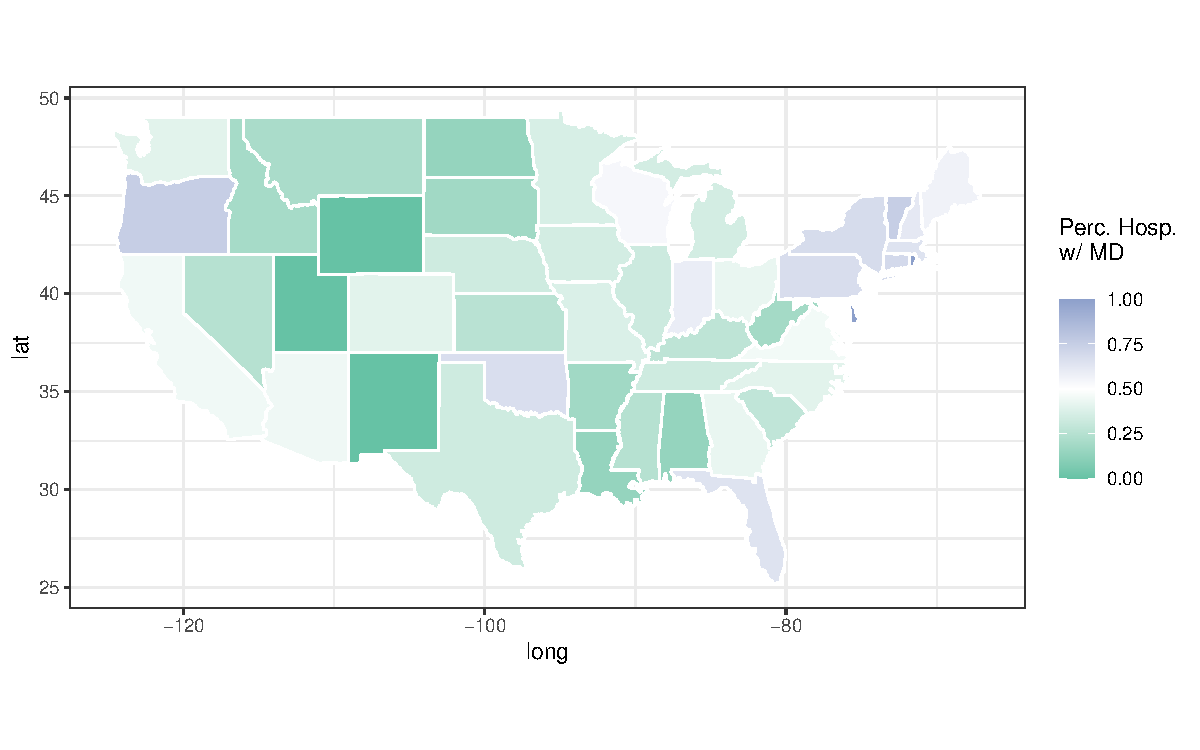
\includegraphics[width=\textwidth]{Objects/has_doc_avg_map.pdf}
    \label{fig:state_doc}
\end{figure}




\section{Matched vs. Unmatched Not-for-Profits}\label{app:matched}

The sample of all NFP hospitals that I use for analysis consists of 852 hospitals. In the AHA data, there are 2,258 additional NFP hospitals that either were not matched to tax forms, did not exist in the tax form data, or did not have executive names in the tax forms. While it would be ideal to analyze all NFPs, a sample size of 852 firms is relatively large in the hospital executive literature. 

In this section, I compare the in-sample NFPs to the out-of-sample NFPs along observable measures. I present means and standard deviations of these measures in Table \ref{tab:nfp_sample_compare}. The in-sample NFPs are slightly larger in terms of beds and patients seen. They are also slightly more likely to be penalized or receive payments under the pay-for-performance incentives. However, average readmission and mortality rates are very similar, as well as case mix index. The largest difference in the two samples is that I under-represent NFP hospitals in systems. This is due to the nature of the tax form 990s, where systems often file one tax form for the entire system, making it difficult to discern the true managers of a specific hospital. Because of this, I drop hospitals from the sample who only have leadership information from a system tax form. 

\import{Tables}{NFP_sample_comparison.tex}





\section{TWFE Regression and Event Study Results}\label{app:fullsample}

While I ultimately employ a synthetic difference-in-differences framework, I also present the coefficient estimates and event study tables under a typical TWFE model specification. That is, there is no weighting of the control group or time periods. Table \ref{tab:forprofit_readmort_fullsample} shows coefficient estimates for the three specifications under Equation \ref{eq:forprofit}. Columns (1)-(3) show coefficient estimates for the weighted average readmission rate outcome, and columns (4)-(6) show coefficient estimates from the weighted average mortality outcome. Generally, these results are qualitatively identical to the synthetic difference-in-difference specification results. There is a statistically significant difference in readmission rate response between for-profits and NFPs with a clinical executive. Specifically, for-profits decrease their readmission rates by .4ppts more than NFPs with a clinical executive. There is no difference (statistically or in magnitude) between readmission rate responses of for-profits compared to all NFPs and NFPs without clincal executives. 

Similarly to the synthetic diff-in-diff estimates, there is no statistical difference in mortality between any of the hospital types, but the magnitude difference between for-profits and NFPs with clinical executives is much larger. This oculd be due to the noisiness of mortality as a measure. 

\import{Tables}{forprofit_readmort_fullsample.tex}

Further, I present coefficient estimates from Equation \ref{eq:clinical} in Table \ref{tab:MD_noMD_readmort_fullsample}, directly comparing NFPs with and without clinical executives for both readmission and mortality rates. Again, these results are very similar to the main results of the paper, with only slightly larger magnitudes. NFPs without a clinical executive respond to the pay-for-performance incentives by decreasing readmission and mortality rates more aggressively than NFPs with clinical executives. 

\import{Tables}{MD_noMD_readmort_fullsample.tex}

Finally, I present these results in typical event study form in Figure \ref{fig:es_plot}, which show no evidence of significant pre-trends driving the findings. 

\begin{figure}[ht!]
     \caption{TWFE Event Study Results}
     \centering
          \begin{subfigure}[b]{0.45\textwidth}
         \centering
         \caption{}
         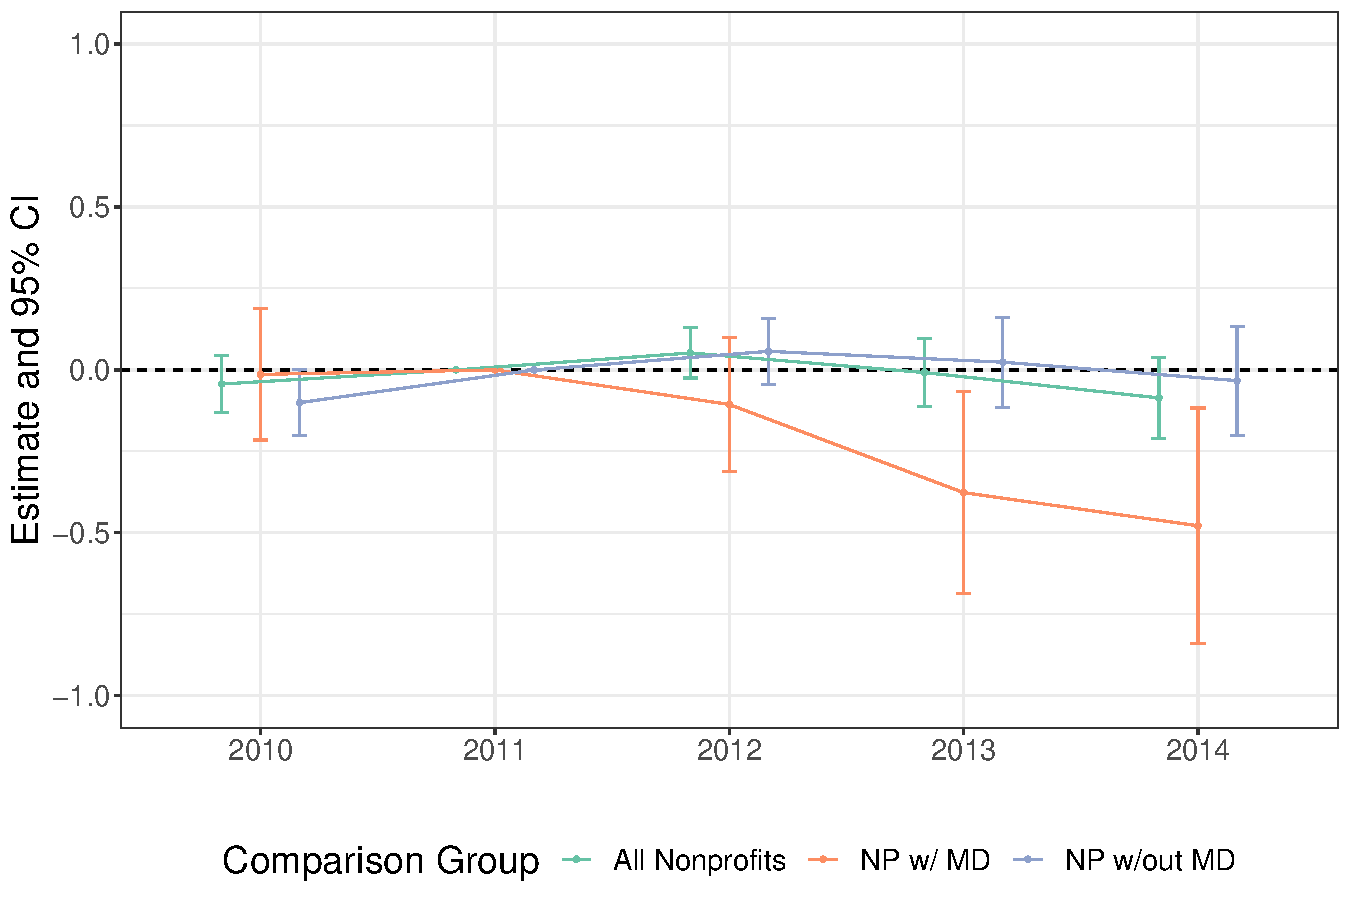
\includegraphics[width=\textwidth]{Objects/read_forprofit_es_graph.pdf}
         \label{fig:es_plota}
     \end{subfigure}%
     \hfill
     \begin{subfigure}[b]{0.45\textwidth}
         \centering
         \caption{}
         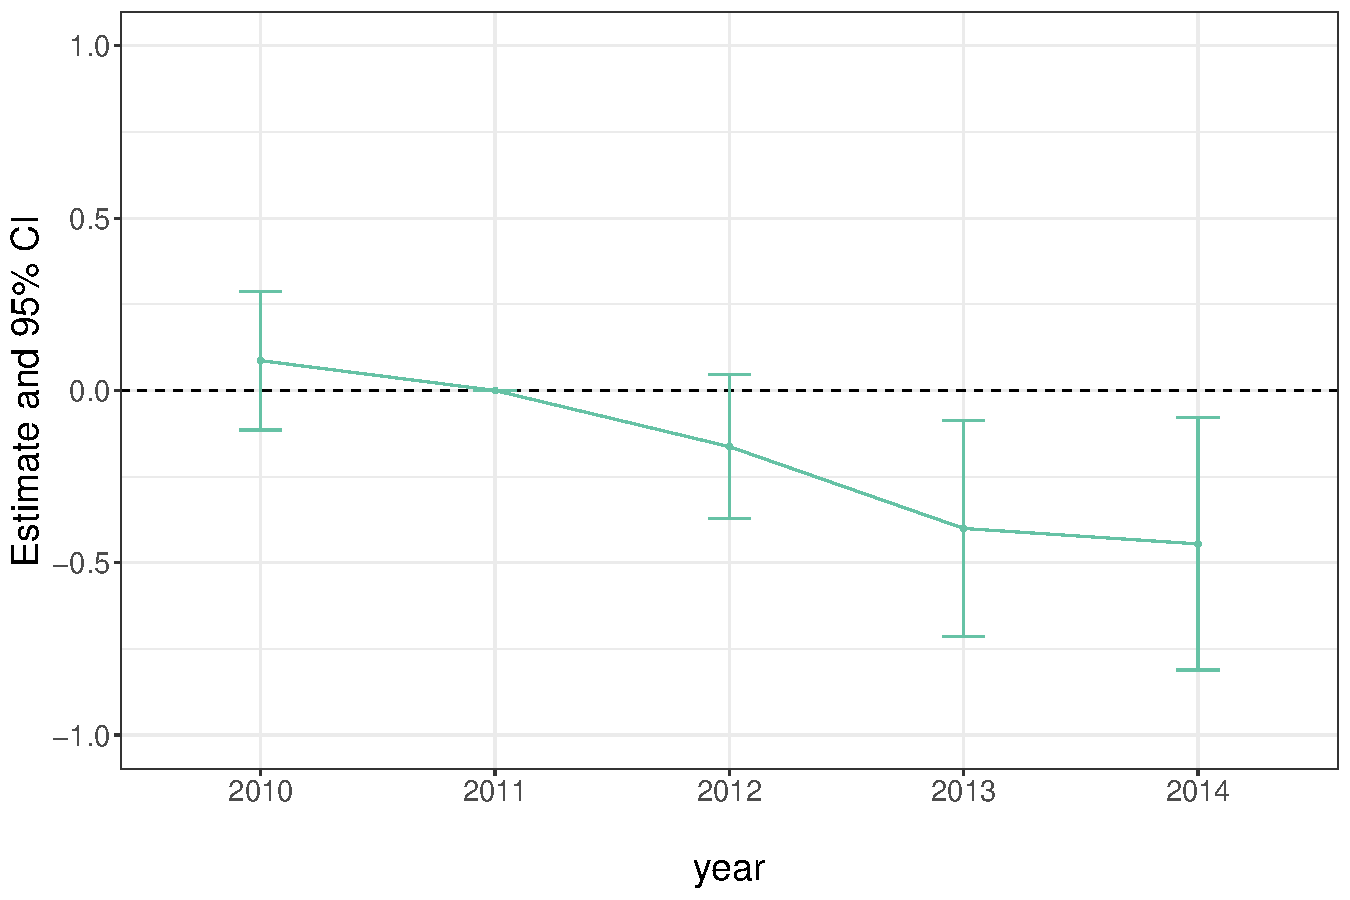
\includegraphics[width=\textwidth]{Objects/read_MD_es_graph.pdf}
         \label{fig:es_plotb}
     \end{subfigure}%
     \vspace{5mm}
     \hfill
     \begin{subfigure}[b]{0.45\textwidth}
         \centering
         \caption{}
         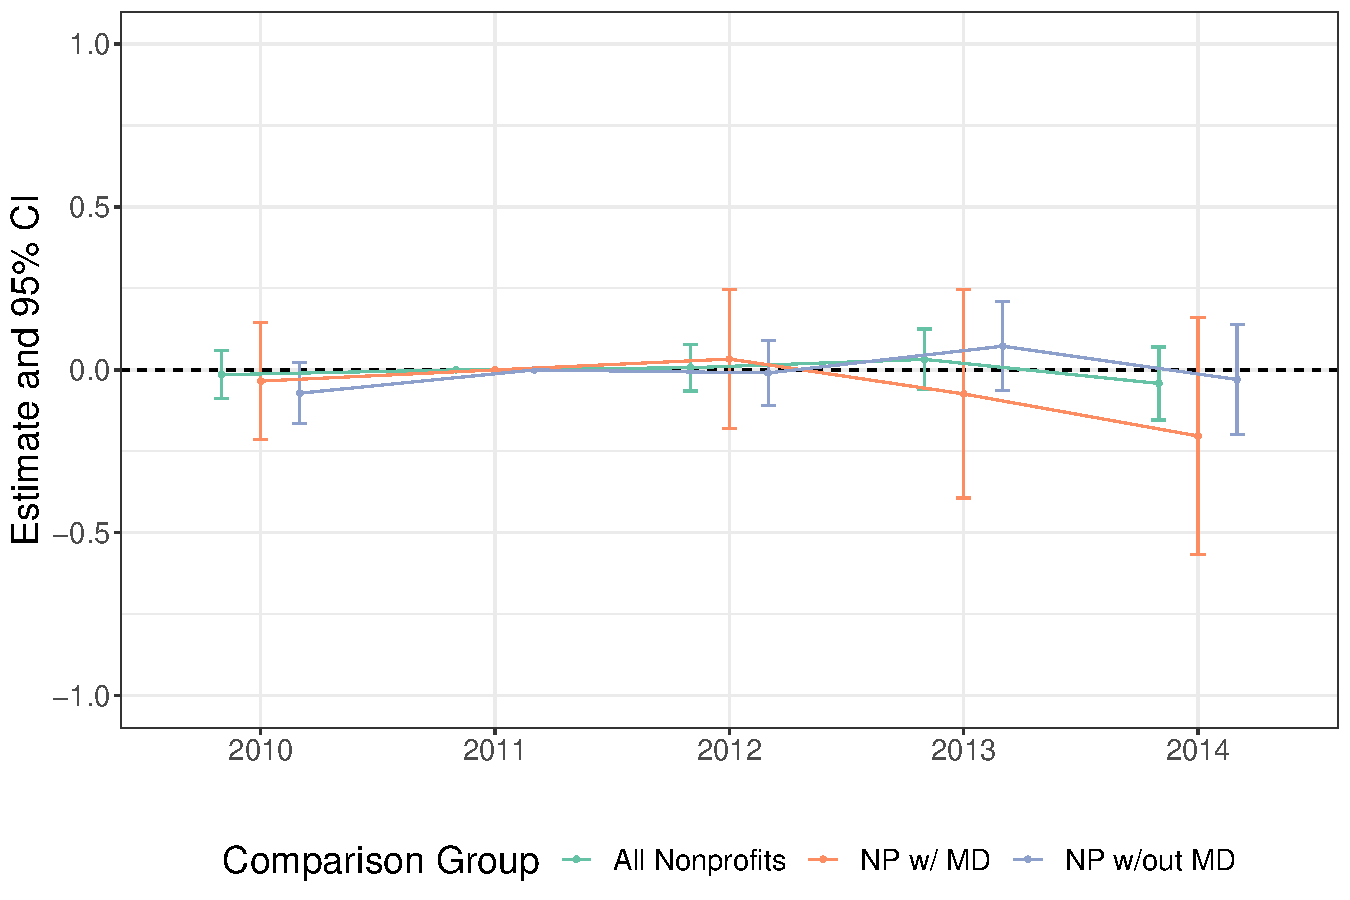
\includegraphics[width=\textwidth]{Objects/mort_forprofit_es_graph.pdf}
         \label{fig:es_plotc}
     \end{subfigure}
     \hfill
     \begin{subfigure}[b]{0.45\textwidth}
         \centering
         \caption{}
         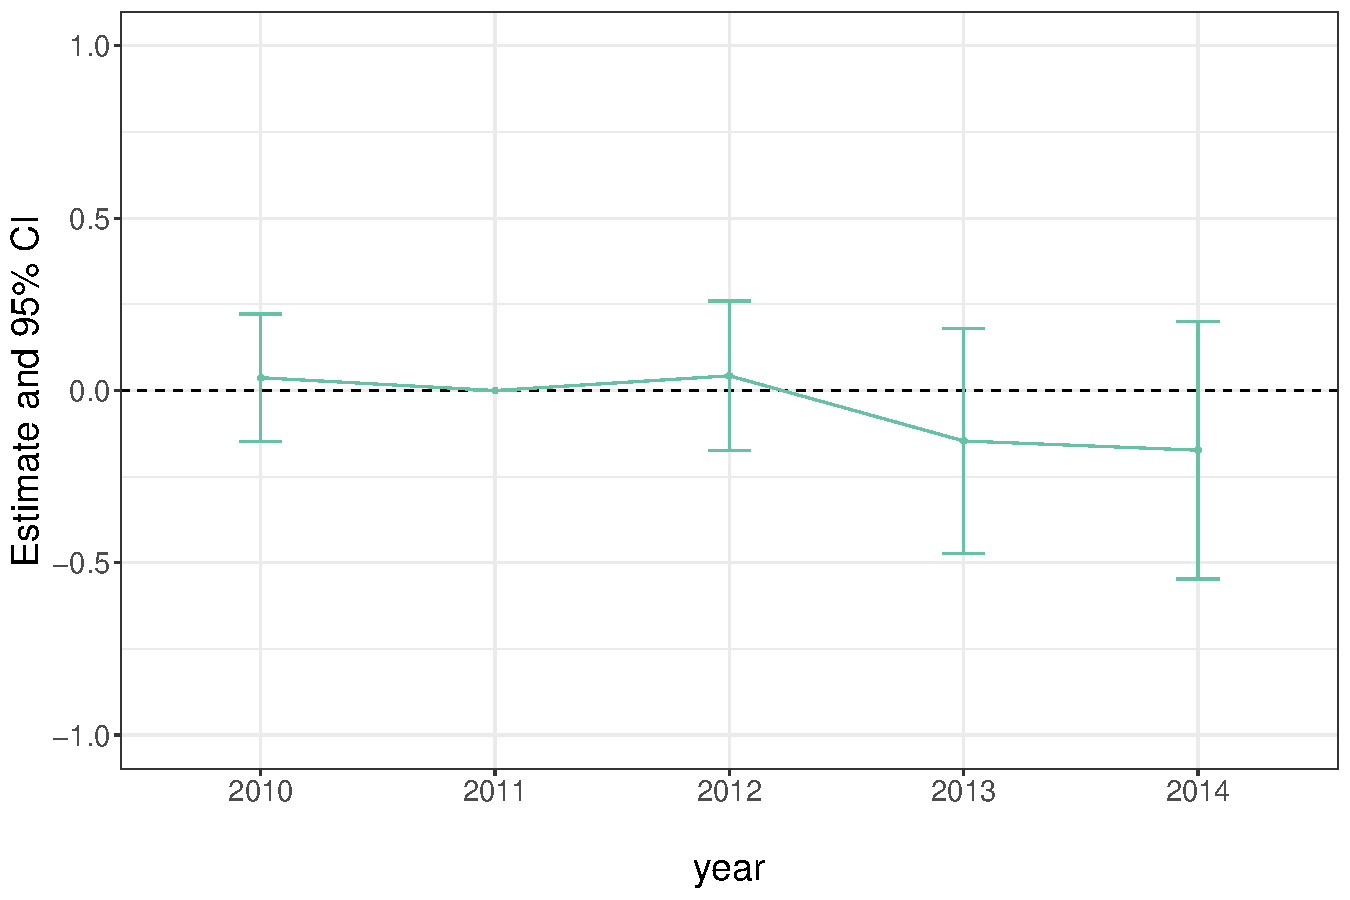
\includegraphics[width=\textwidth]{Objects/mort_MD_es_graph.pdf}
         \label{fig:es_plotd}
     \end{subfigure}
        \label{fig:es_plot}
    \end{figure}




\section{Synthetic Difference-in-Difference Coefficient Tables}

While I present the graphical representation of results in the main text, I also present a table of coefficients and standard errors for readmission and mortality rates in Tables \ref{tab:forprofit_readmort_synth} and \ref{tab:MD_noMD_readmort_synth}.

\import{Tables}{forprofit_readmort_synth.tex}

\import{Tables}{MD_noMD_readmort_synth.tex}


    

    

    

    

    

    

	
	
	


\end{document}

